\documentclass[11pt,preprint, authoryear]{elsarticle}

\usepackage{lmodern}
%%%% My spacing
\usepackage{setspace}
\setstretch{1.2}
\DeclareMathSizes{12}{14}{10}{10}

% Wrap around which gives all figures included the [H] command, or places it "here". This can be tedious to code in Rmarkdown.
\usepackage{float}
\let\origfigure\figure
\let\endorigfigure\endfigure
\renewenvironment{figure}[1][2] {
    \expandafter\origfigure\expandafter[H]
} {
    \endorigfigure
}

\let\origtable\table
\let\endorigtable\endtable
\renewenvironment{table}[1][2] {
    \expandafter\origtable\expandafter[H]
} {
    \endorigtable
}


\usepackage{ifxetex,ifluatex}
\usepackage{fixltx2e} % provides \textsubscript
\ifnum 0\ifxetex 1\fi\ifluatex 1\fi=0 % if pdftex
  \usepackage[T1]{fontenc}
  \usepackage[utf8]{inputenc}
\else % if luatex or xelatex
  \ifxetex
    \usepackage{mathspec}
    \usepackage{xltxtra,xunicode}
  \else
    \usepackage{fontspec}
  \fi
  \defaultfontfeatures{Mapping=tex-text,Scale=MatchLowercase}
  \newcommand{\euro}{€}
\fi

\usepackage{amssymb, amsmath, amsthm, amsfonts}

\def\bibsection{\section*{References}} %%% Make "References" appear before bibliography


\usepackage[round]{natbib}

\usepackage{longtable}
\usepackage[margin=2.3cm,bottom=2cm,top=2.5cm, includefoot]{geometry}
\usepackage{fancyhdr}
\usepackage[bottom, hang, flushmargin]{footmisc}
\usepackage{graphicx}
\numberwithin{equation}{section}
\numberwithin{figure}{section}
\numberwithin{table}{section}
\setlength{\parindent}{0cm}
\setlength{\parskip}{1.3ex plus 0.5ex minus 0.3ex}
\usepackage{textcomp}
\renewcommand{\headrulewidth}{0.2pt}
\renewcommand{\footrulewidth}{0.3pt}

\usepackage{array}
\newcolumntype{x}[1]{>{\centering\arraybackslash\hspace{0pt}}p{#1}}

%%%%  Remove the "preprint submitted to" part. Don't worry about this either, it just looks better without it:
\makeatletter
\def\ps@pprintTitle{%
  \let\@oddhead\@empty
  \let\@evenhead\@empty
  \let\@oddfoot\@empty
  \let\@evenfoot\@oddfoot
}
\makeatother

 \def\tightlist{} % This allows for subbullets!

\usepackage{hyperref}
\hypersetup{breaklinks=true,
            bookmarks=true,
            colorlinks=true,
            citecolor=blue,
            urlcolor=blue,
            linkcolor=blue,
            pdfborder={0 0 0}}


% The following packages allow huxtable to work:
\usepackage{siunitx}
\usepackage{multirow}
\usepackage{hhline}
\usepackage{calc}
\usepackage{tabularx}
\usepackage{booktabs}
\usepackage{caption}


\newenvironment{columns}[1][]{}{}

\newenvironment{column}[1]{\begin{minipage}{#1}\ignorespaces}{%
\end{minipage}
\ifhmode\unskip\fi
\aftergroup\useignorespacesandallpars}

\def\useignorespacesandallpars#1\ignorespaces\fi{%
#1\fi\ignorespacesandallpars}

\makeatletter
\def\ignorespacesandallpars{%
  \@ifnextchar\par
    {\expandafter\ignorespacesandallpars\@gobble}%
    {}%
}
\makeatother

\newlength{\cslhangindent}
\setlength{\cslhangindent}{1.5em}
\newenvironment{CSLReferences}%
  {\setlength{\parindent}{0pt}%
  \everypar{\setlength{\hangindent}{\cslhangindent}}\ignorespaces}%
  {\par}


\urlstyle{same}  % don't use monospace font for urls
\setlength{\parindent}{0pt}
\setlength{\parskip}{6pt plus 2pt minus 1pt}
\setlength{\emergencystretch}{3em}  % prevent overfull lines
\setcounter{secnumdepth}{5}

%%% Use protect on footnotes to avoid problems with footnotes in titles
\let\rmarkdownfootnote\footnote%
\def\footnote{\protect\rmarkdownfootnote}
\IfFileExists{upquote.sty}{\usepackage{upquote}}{}

%%% Include extra packages specified by user

%%% Hard setting column skips for reports - this ensures greater consistency and control over the length settings in the document.
%% page layout
%% paragraphs
\setlength{\baselineskip}{12pt plus 0pt minus 0pt}
\setlength{\parskip}{12pt plus 0pt minus 0pt}
\setlength{\parindent}{0pt plus 0pt minus 0pt}
%% floats
\setlength{\floatsep}{12pt plus 0 pt minus 0pt}
\setlength{\textfloatsep}{20pt plus 0pt minus 0pt}
\setlength{\intextsep}{14pt plus 0pt minus 0pt}
\setlength{\dbltextfloatsep}{20pt plus 0pt minus 0pt}
\setlength{\dblfloatsep}{14pt plus 0pt minus 0pt}
%% maths
\setlength{\abovedisplayskip}{12pt plus 0pt minus 0pt}
\setlength{\belowdisplayskip}{12pt plus 0pt minus 0pt}
%% lists
\setlength{\topsep}{10pt plus 0pt minus 0pt}
\setlength{\partopsep}{3pt plus 0pt minus 0pt}
\setlength{\itemsep}{5pt plus 0pt minus 0pt}
\setlength{\labelsep}{8mm plus 0mm minus 0mm}
\setlength{\parsep}{\the\parskip}
\setlength{\listparindent}{\the\parindent}
%% verbatim
\setlength{\fboxsep}{5pt plus 0pt minus 0pt}



\begin{document}



\begin{frontmatter}  %

\title{Question Two}

% Set to FALSE if wanting to remove title (for submission)




\author[Add1]{Jessica Van der Berg}
\ead{20190565@sun.ac.za}





\address[Add1]{Financial Econometrics, 2021}


\begin{abstract}
\small{
This document contains the detailed answers for question two of the
Financial Econometric exam 2021.
}
\end{abstract}

\vspace{1cm}


\begin{keyword}
\footnotesize{
Question2\sep Finance \sep Financial Econometrics \\
\vspace{0.3cm}
}
\footnotesize{
\textit{JEL classification} L250 \sep L100
}
\end{keyword}



\vspace{0.5cm}

\end{frontmatter}



%________________________
% Header and Footers
%%%%%%%%%%%%%%%%%%%%%%%%%%%%%%%%%
\pagestyle{fancy}
\chead{}
\rhead{}
\lfoot{}
\rfoot{\footnotesize Page \thepage}
\lhead{}
%\rfoot{\footnotesize Page \thepage } % "e.g. Page 2"
\cfoot{}

%\setlength\headheight{30pt}
%%%%%%%%%%%%%%%%%%%%%%%%%%%%%%%%%
%________________________

\headsep 35pt % So that header does not go over title




\hypertarget{caparing-swix-and-alsi}{%
\section{Caparing SWIX and ALSI}\label{caparing-swix-and-alsi}}

\hypertarget{portfolio-return}{%
\subsection{Portfolio Return}\label{portfolio-return}}

The porfolio returns for large and mid caps are shown below. Because we
are analyzing the Top 40, there are no small caps, and if there are,
they make up such a small percentage of the portfolio that it makes no
sense to analyze them.

The graph for Mid caps return saw very constant returns up until mid
year, 2017. Afterwhich it experienced a slight increase followed by a
drastic decrease. This would be an indication of an negative, al though
constant investment. Investors that are looking for a high return is
unlikely to experience this. The SWIX outperforms the ALSI, which is a
preference for when the market is constant/slight increase. However,
during negative volatility, the SWIX performs worse. It is important to
remember that mid-cap companies can turn into large-cap companies, which
also make them attractive to investors. However, you will need to spot
the diamond in the rough.
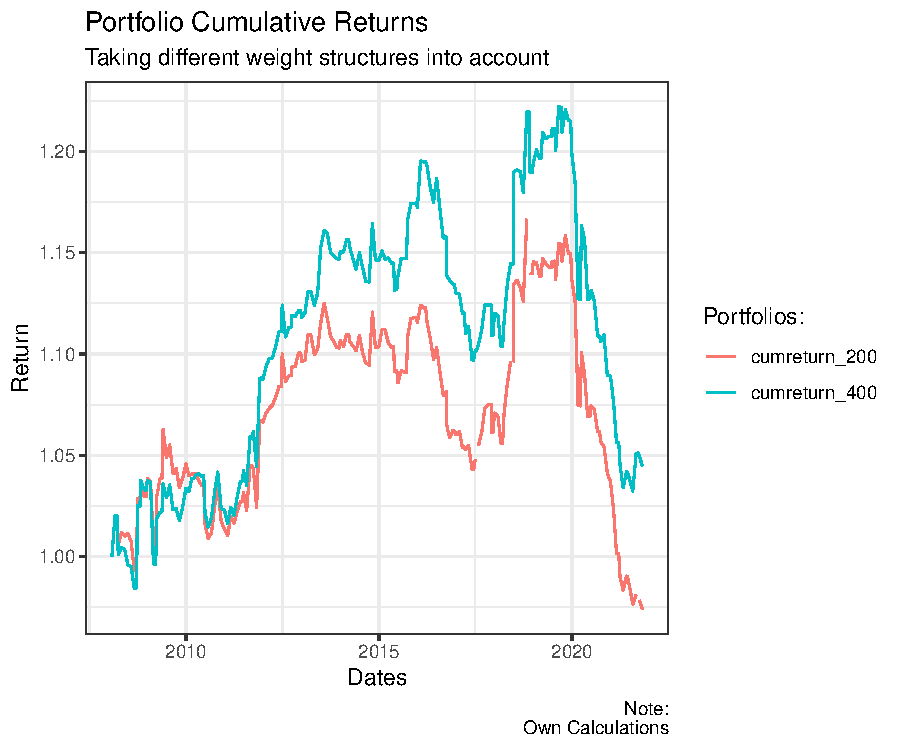
\includegraphics{Question2_files/figure-latex/unnamed-chunk-1-1.pdf} The
portfolio cumulative returns for Large Caps experience much more
volatility then Mid Caps. Large Caps are filled with companies that are
dominate in their industry, and while they are still affect by
volatility, they have more of a chance to bounce back. They hold
themselves well in times of recession or during any other negative
event. Besides, they will usually have been functioning for decades and
have good reputations. If you want to invest in a companies stocks by
taking less risk, then large-cap stocks are a good option. These stocks
are less volatile in comparison to mid-cap. The lower volatility makes
them less risky.

As seen in th graph below, Large caps present a higher return, but also
experienced a downturn with the depletion of economic events in 2020.

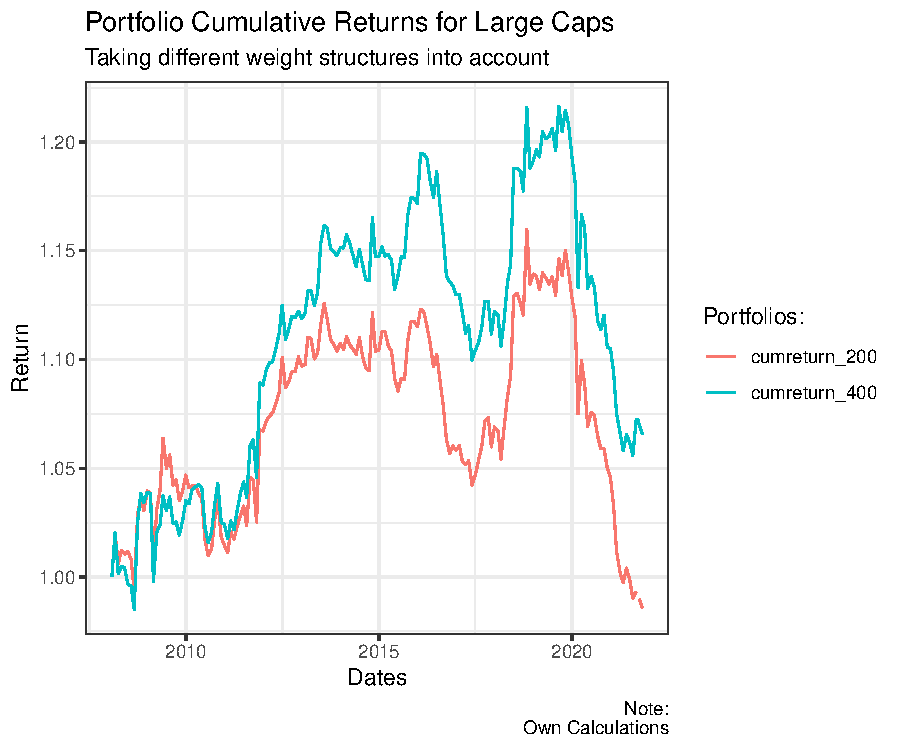
\includegraphics{Question2_files/figure-latex/unnamed-chunk-2-1.pdf}
\#\#\# Sector Analysis

The industrial sector has preformed relatively well compared to the
financial sector (discussed below). The sector has been on an increasing
trend with the COVID-19 pandemic resulting in slowdown and negative
growth.

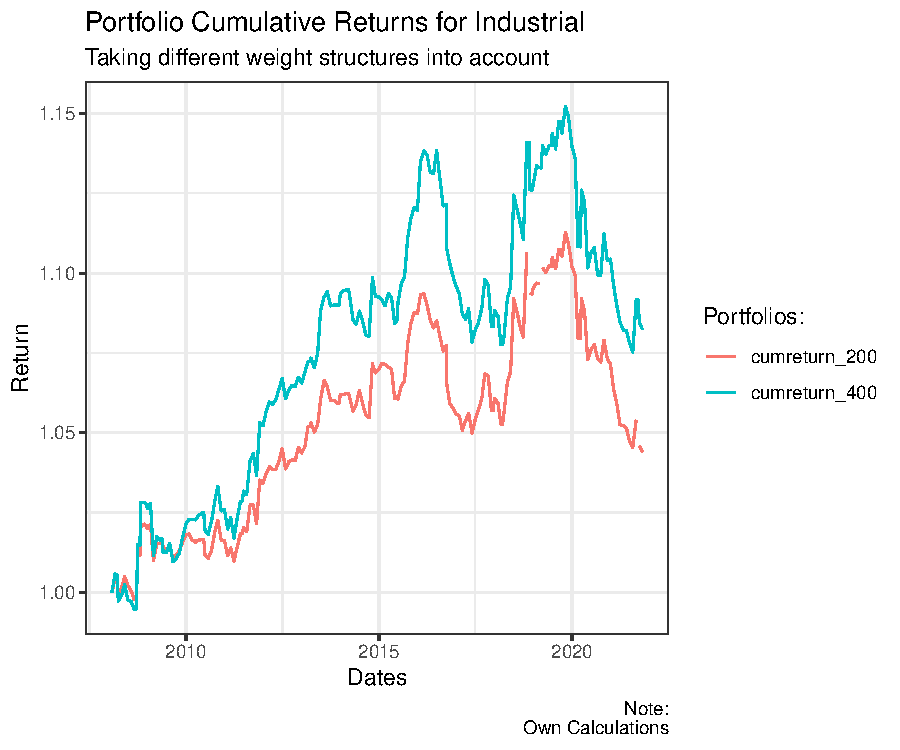
\includegraphics{Question2_files/figure-latex/unnamed-chunk-3-1.pdf} The
graph below for the financial structure looks very similar to that of
the large-caps (which was discussed above). This indicates that many of
the financial sector companies that are being analyzed are large-cap
companies. This implies that even though a sharp decrease can be seen,
these companies have a high probability to bounce back.

There are have been some aggressive monetary and fiscal policy responses
to the COVID-19 pandemic, which would contribute towards stabilizing the
market and ensuring the industry starts growing again.
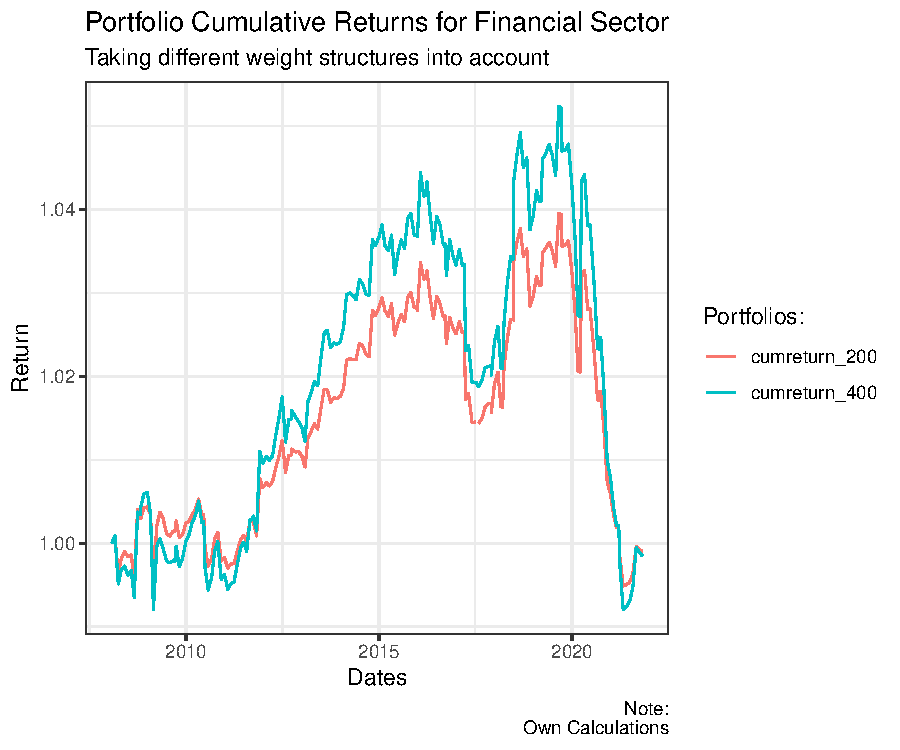
\includegraphics{Question2_files/figure-latex/unnamed-chunk-4-1.pdf}
\#\# Staritication

I use the only the index from 2008 onwards since this is the only data
that is available.

\hypertarget{caping}{%
\subsection{Caping}\label{caping}}

I capped the SWIX to 6 percent and the ALSI to 10 percent (this is how I
interpreted the question). I couldn.t get the cap exactly right but I
think I was on the right path

\bibliography{Tex/ref}





\end{document}
